\section{Data Results}
After closure of the background estimation procedure within the control region \ref{sec:bssecondsideband}, we investigate signal region.  
The results in the signal region are shown in Figure \ref{figs:bsMtwvsBkg1}.  We proceed to compute 
limits on the $\bs$ cross-section.  Background estimation of selected relevant variables can be seen in 
Figures \ref{figs:bskinplotsdata1} and \ref{figs:bskinplotsdata2}.

The expected number of events in the signal region is 359 $\pm$ 58, the observed number of events is 318.  Table \ref{table:bssigeff} gives the signal efficiency in the signal region for 
the three signal coupling hypotheses.

\begin{table}
\begin{center}
\bf{$\bs$ signal region efficiency}\\
\begin{tabular}{c||c|c|c}
\hline\hline
\bf{$\mathrm{M_{\bs}}$} & \bf{$\epsilon_{R}$}  & \bf{$\epsilon_{L}$} & \bf{$\epsilon_{LR}$} \\
\hline\hline
800 & 0.0014 & 0.0010 & 0.0012\\
900 & 0.0076 & 0.0063 & 0.0070\\
1000 & 0.0301 & 0.0243 & 0.0272\\
1100 & 0.0502 & 0.0411 & 0.0456\\
1200 & 0.0653 & 0.0522 & 0.0588\\
1300 & 0.0746 & 0.0590 & 0.0668\\
1400 & 0.0788 & 0.0636 & 0.0712\\
1500 & 0.0809 & 0.0629 & 0.0719\\
1600 & 0.0795 & 0.0616 & 0.0706\\
1700 & 0.0760 & 0.0596 & 0.0678\\
1800 & 0.0749 & 0.0569 & 0.0659\\
1900 & 0.0707 & 0.0536 & 0.0622\\
2000 & 0.0660 & 0.0499 & 0.0583\\
\hline
\end{tabular}
\end{center}
\caption{$\bs$ signal efficiency for left-handed, right-handed and vectorlike $\bs$ samples}
\label{table:bssigeff}
\end{table}





\begin{figure}[htcb]
\begin{center}
\subfigure{\label{figs:bsMtwvsBkg_BifPoly_fit}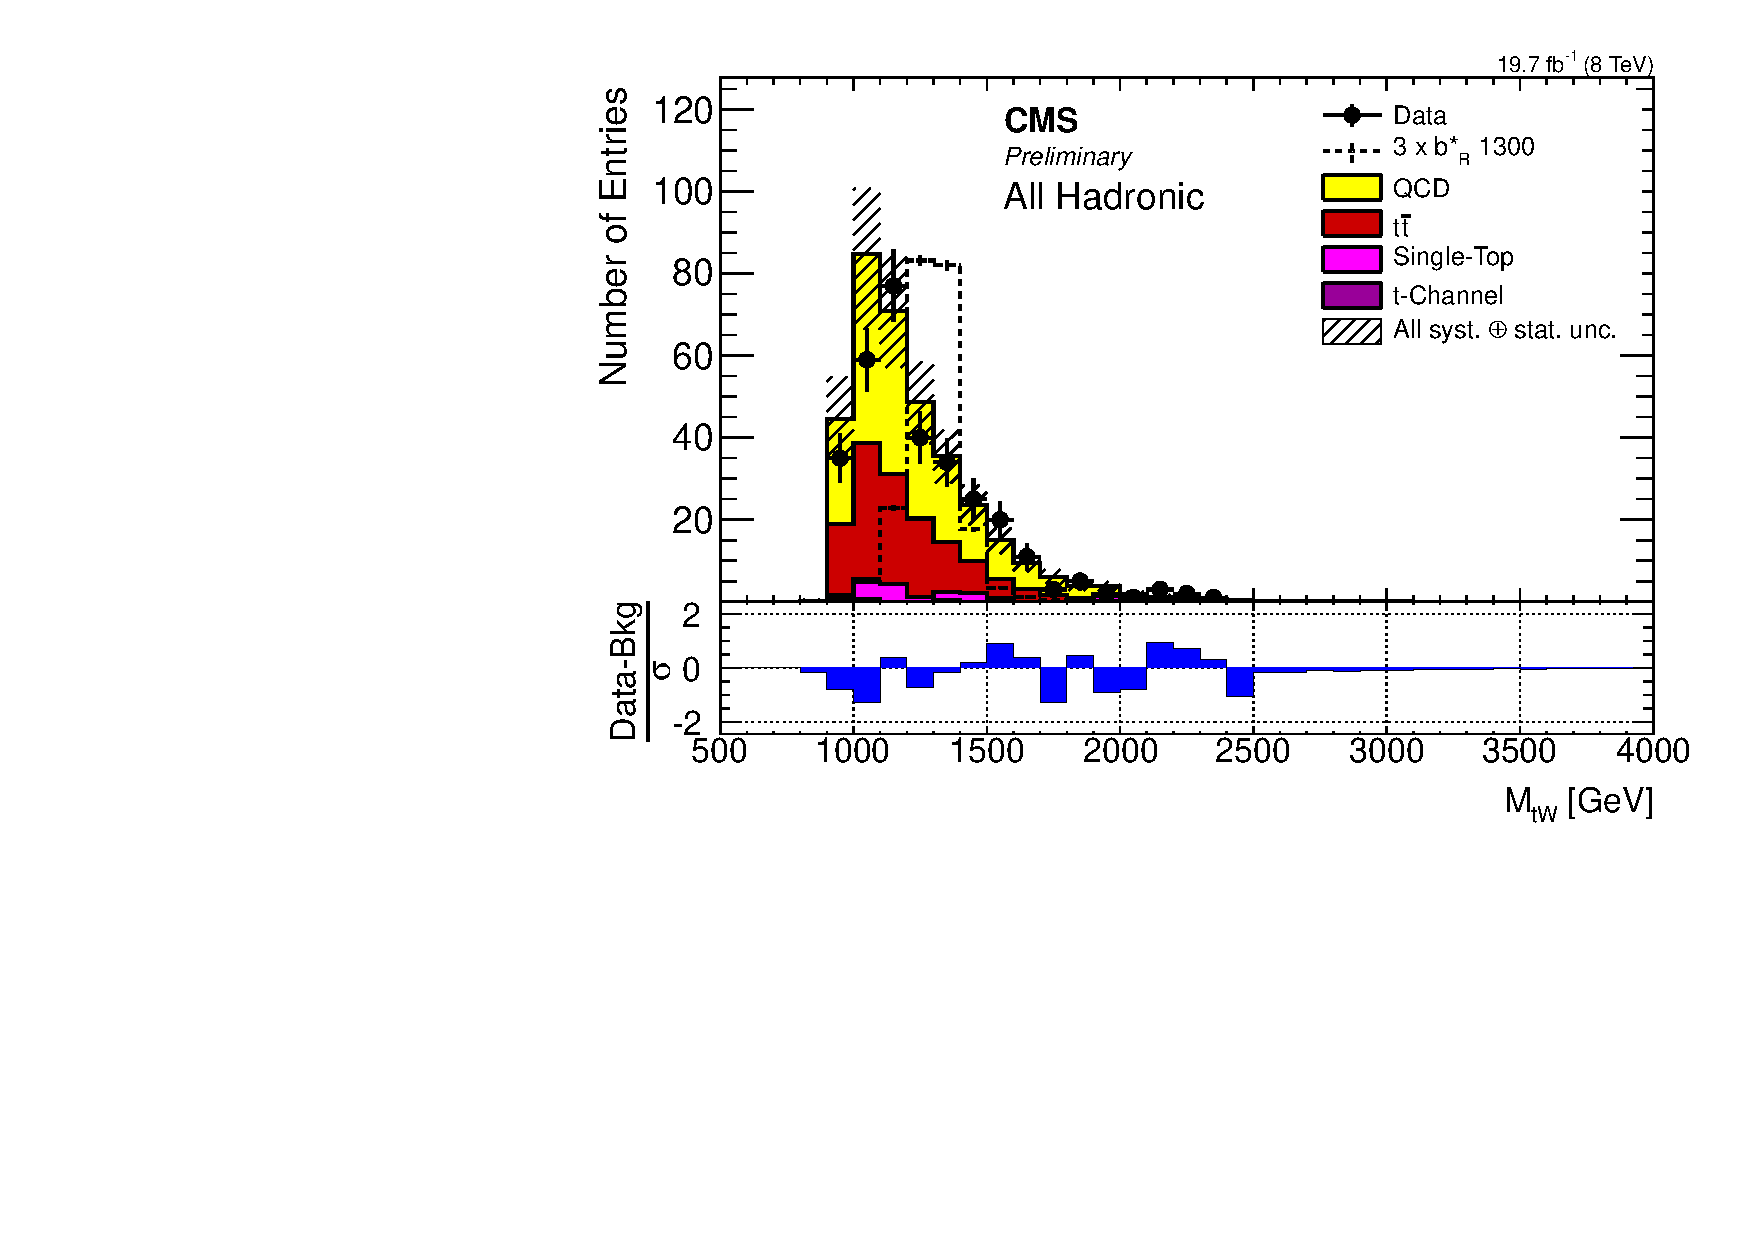
\includegraphics[width=0.7\textwidth]{AN-14-049/figs/MtwvsBkg_BifPoly_fit.pdf}}\\
\subfigure{\label{figs:bsMtwvsBkgsemilog_BifPoly_fit}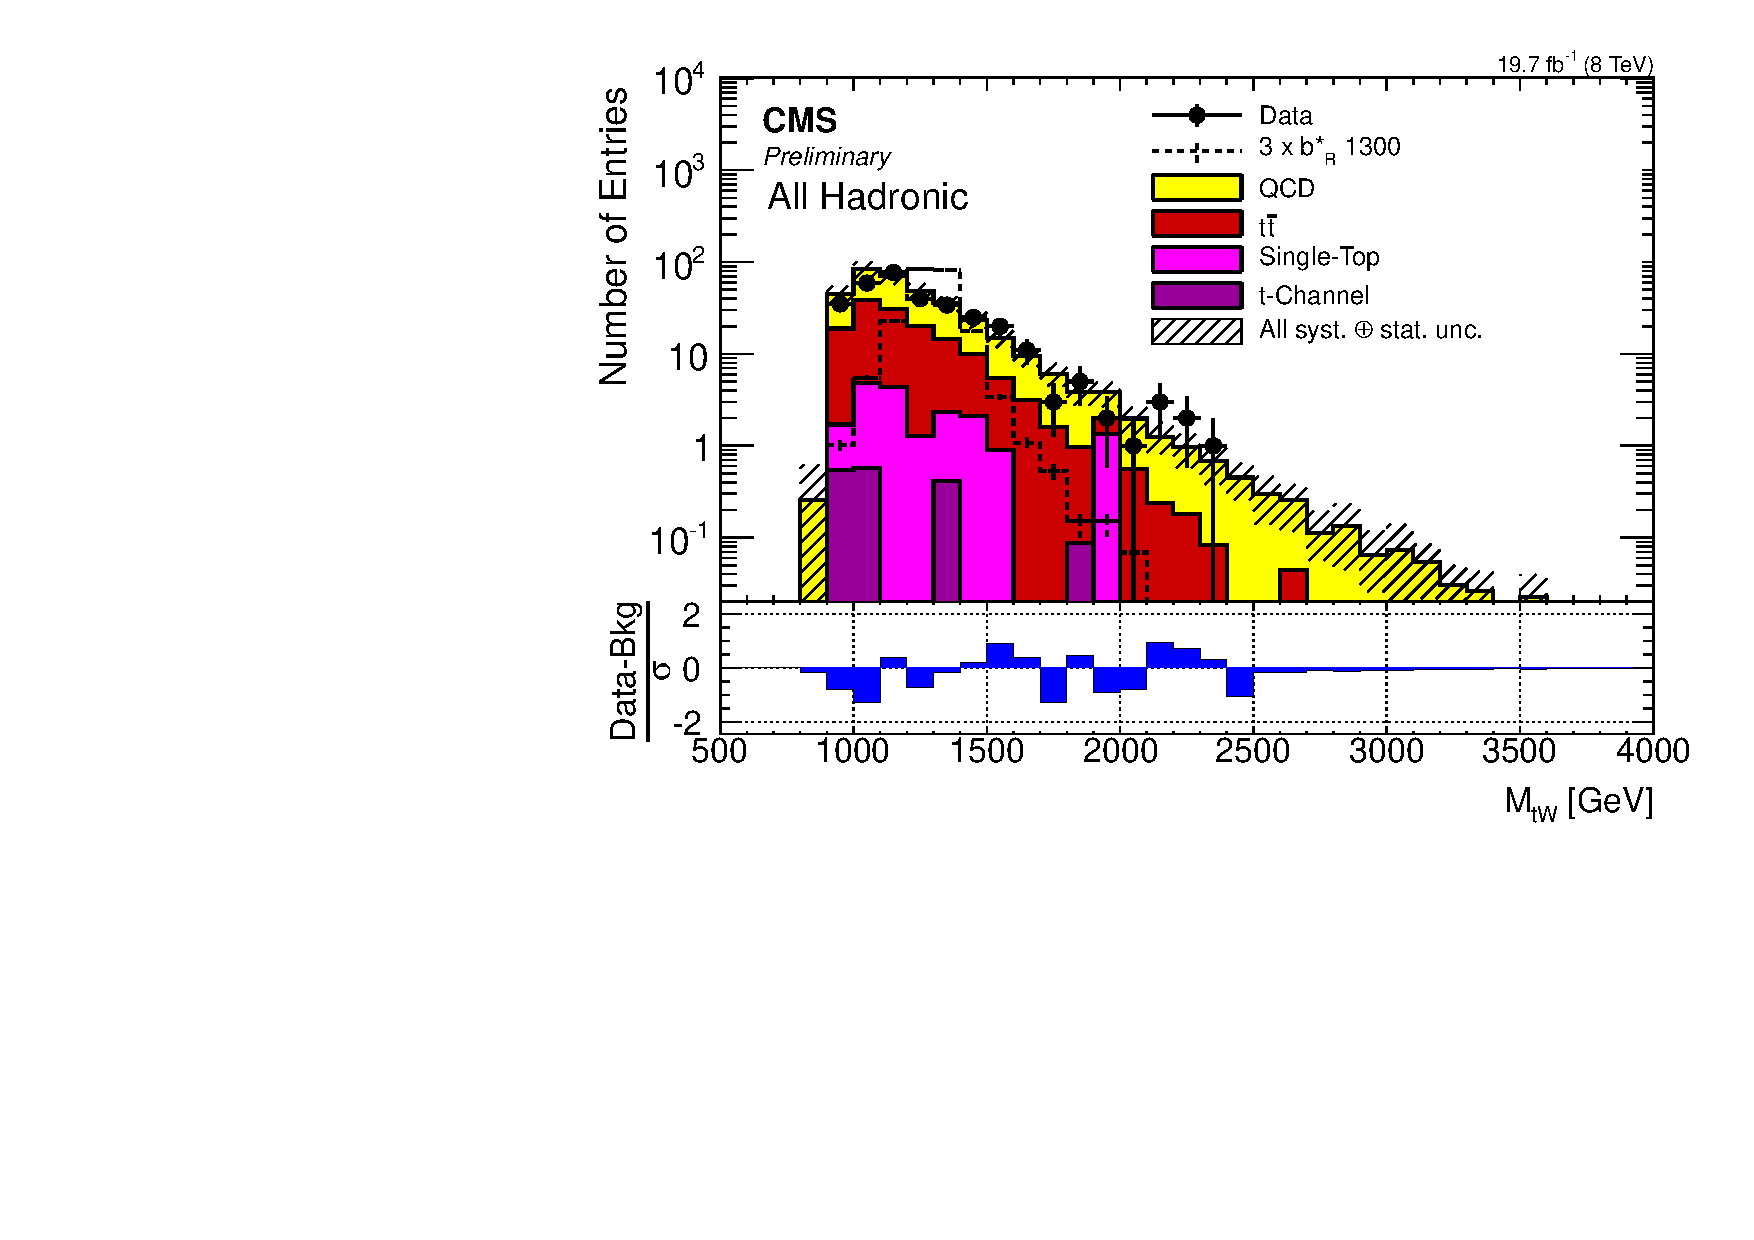
\includegraphics[width=0.7\textwidth]{AN-14-049/figs/MtwvsBkgsemilog_BifPoly_fit.pdf}}
\caption{
A plot of the full selection comparing data, signal and background.  
Top and bottom plots are the same but on linear and log y-axis scale.}
\label{figs:bsMtwvsBkg1}
\end{center}
\end{figure}

\begin{figure}[htcb]
\centering
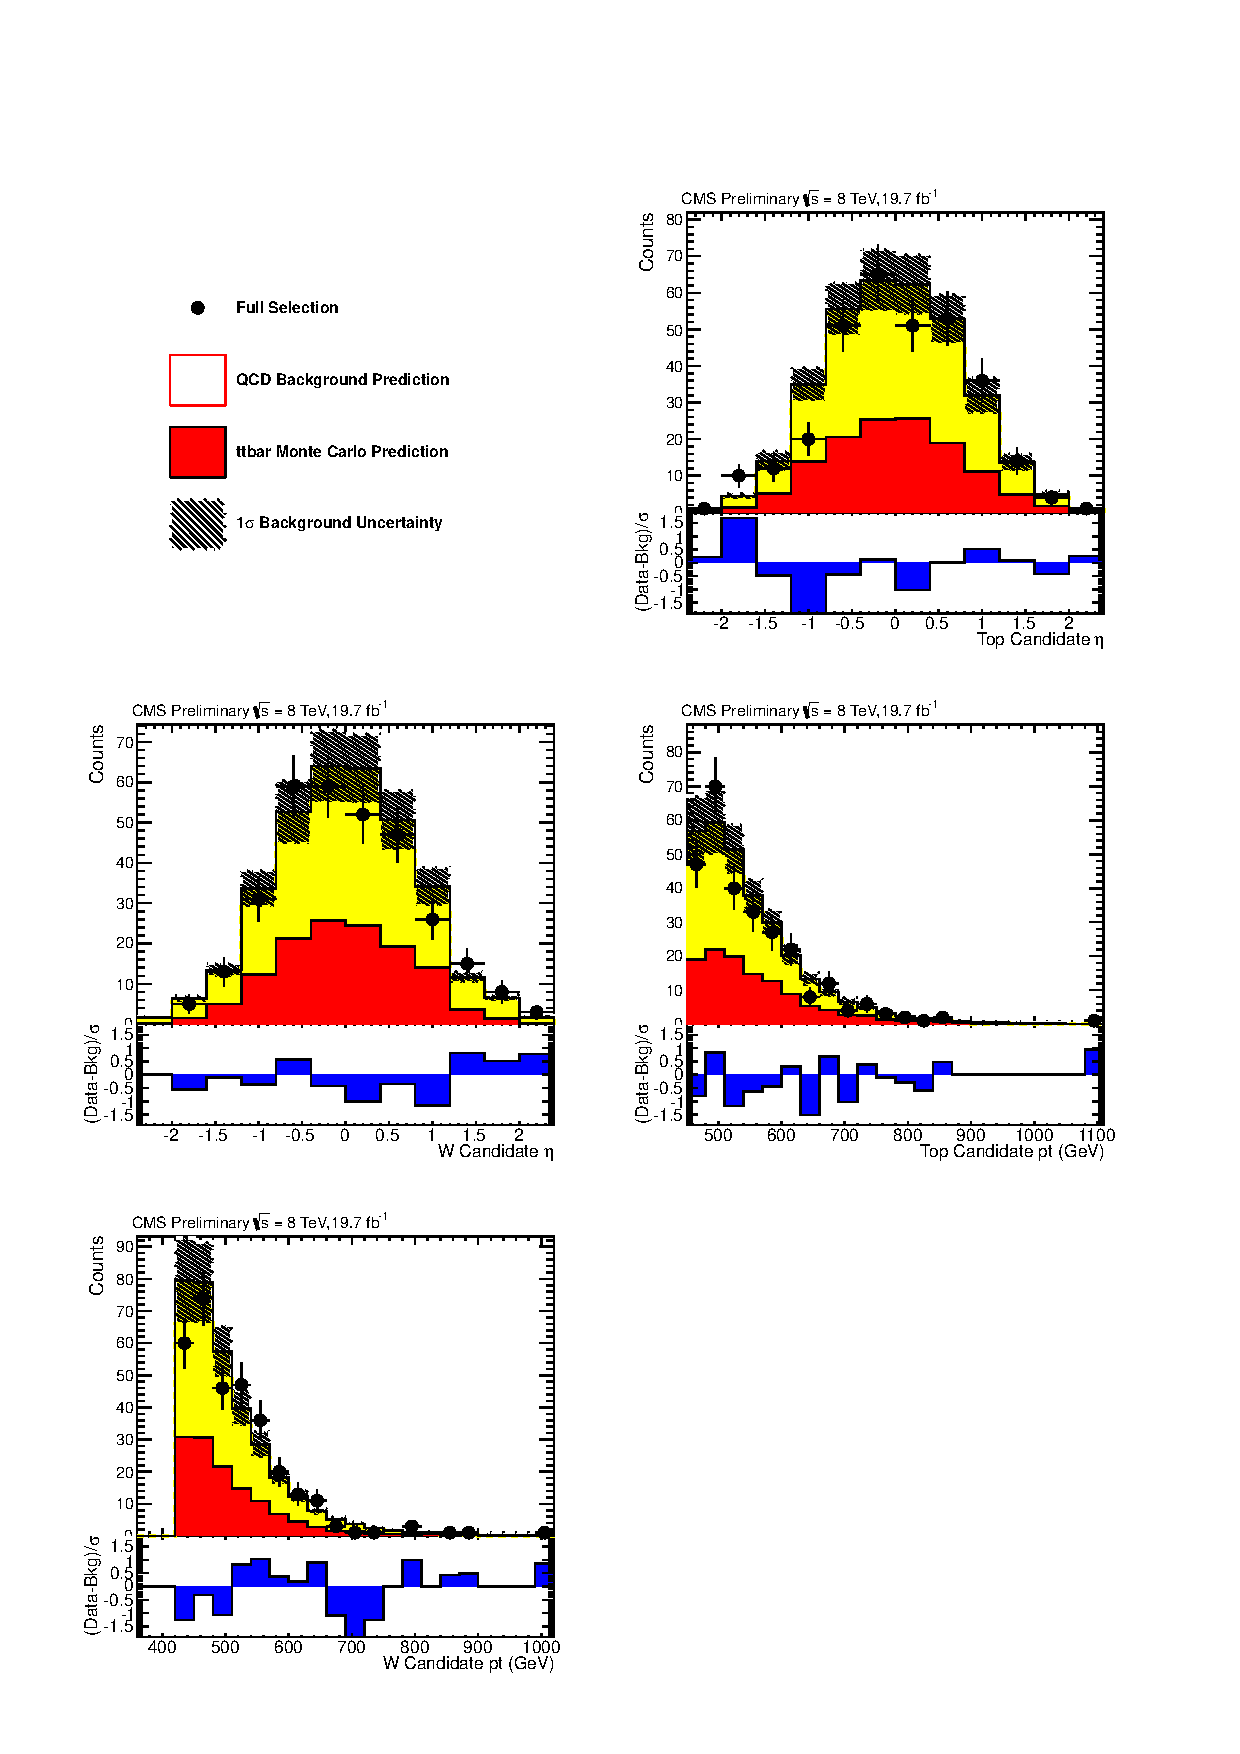
\includegraphics[width=.7\textwidth]{AN-14-049/figs/KinPlots_Data1.pdf}
\caption{Background estimation of kinematic variables.  
The error bars shown are from the three primary sources; uncertainty on the fit, choice of fit, top mass modification, $\ttbar$ normalization, and $\ttbar$ $Q^2$ uncertainty}
\label{figs:bskinplotsdata1}
\end{figure}  
\clearpage

\begin{figure}[htcb]
\centering
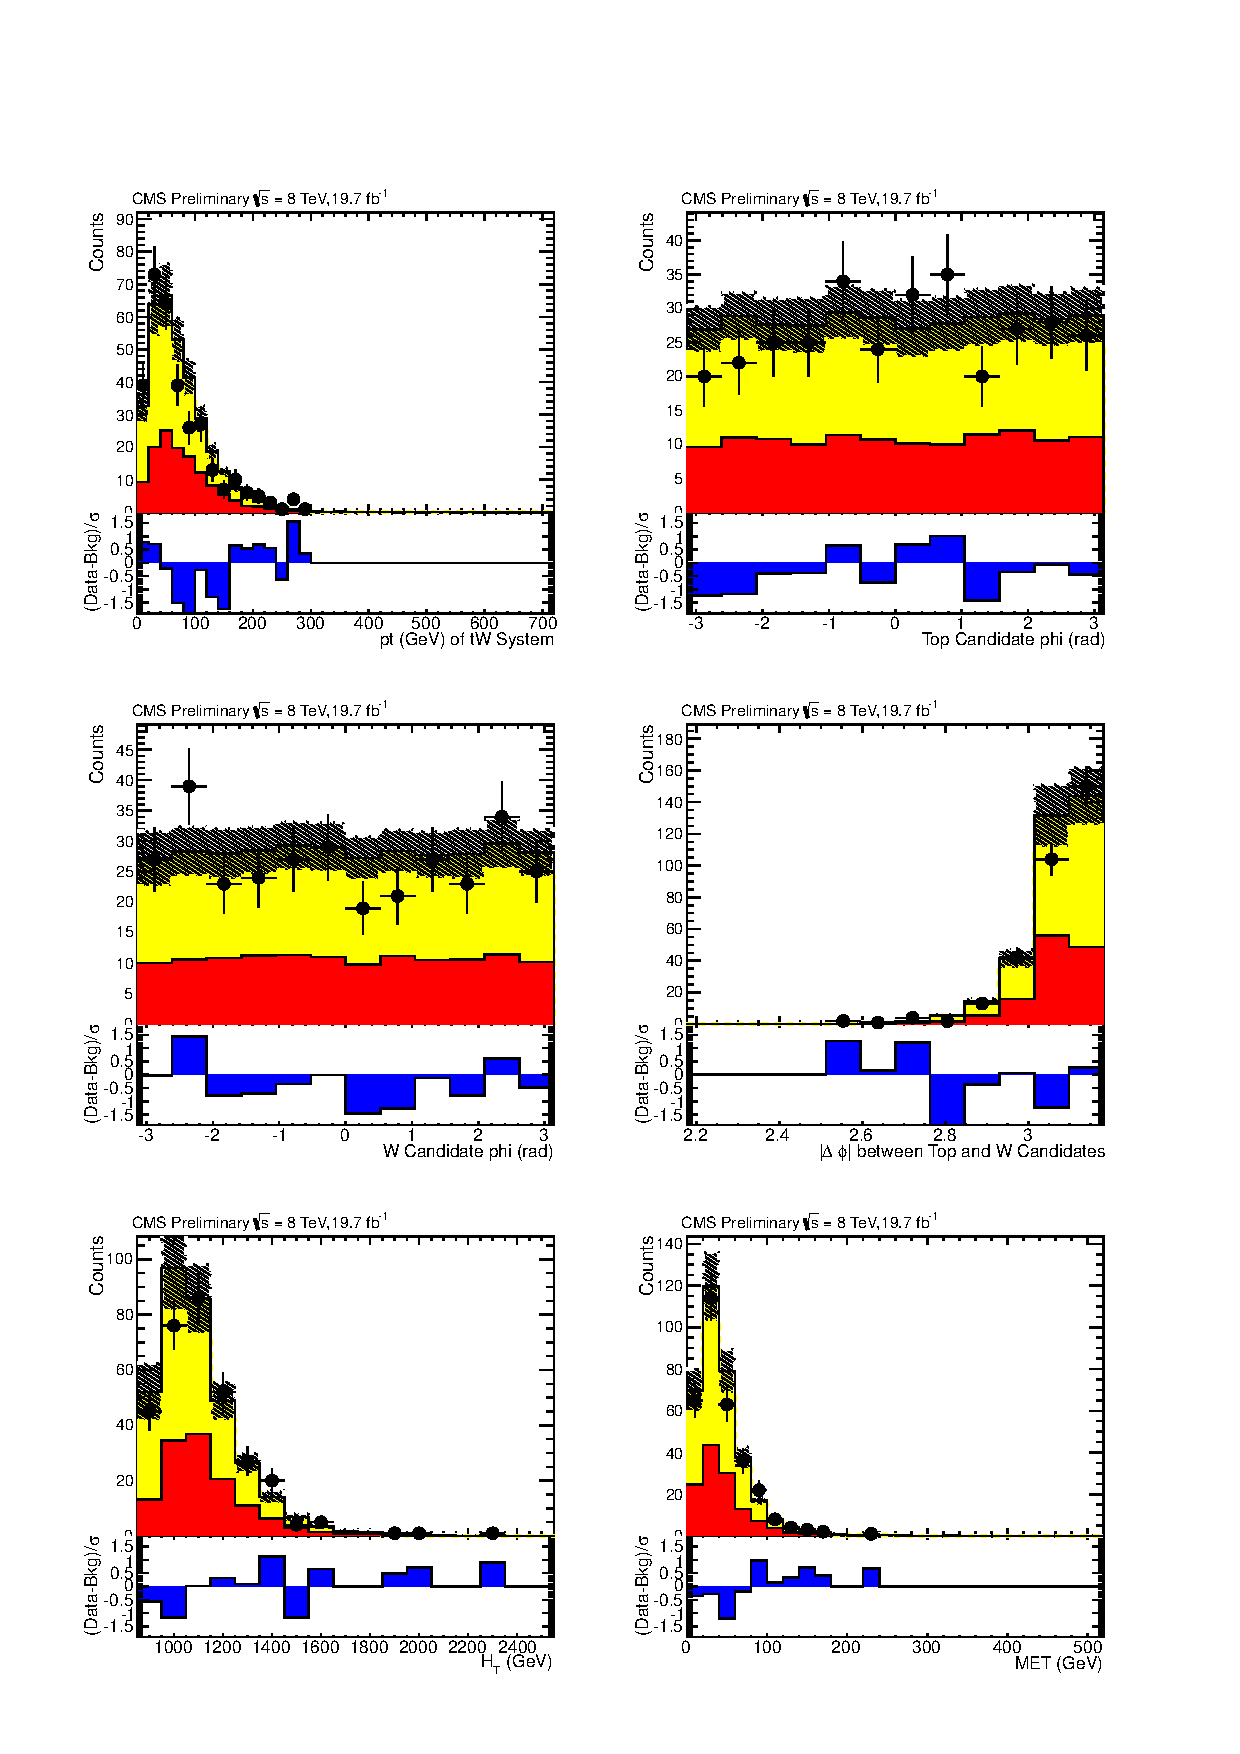
\includegraphics[width=.7\textwidth]{AN-14-049/figs/KinPlots_Data2.pdf}
\caption{Background estimation of kinematic variables.  
The error bars shown are from the three primary sources; uncertainty on the fit, choice of fit, top mass modification, $\ttbar$ normalization, and $\ttbar$ $Q^2$ uncertainty}
\label{figs:bskinplotsdata2}
\end{figure}  
\clearpage

